\documentclass{article}

\usepackage{tikzfig}
\usepackage{amsmath}
\usepackage{amssymb}
\usepackage{stmaryrd}
\usepackage{amsthm}
\usepackage{xspace}
\usepackage{hyperref}
\usepackage{graphicx}
\graphicspath{{figures/}}

\usepackage{algpseudocode}
\usepackage{algorithm}

\newtheorem{theorem}{Theorem}[section]
\newtheorem*{theorem*}{Theorem}
\newtheorem{proposition}[theorem]{Proposition}
\newtheorem{lemma}[theorem]{Lemma}
\newtheorem{corollary}[theorem]{Corollary}
\theoremstyle{definition}\newtheorem{example}[theorem]{Example}
\theoremstyle{definition}\newtheorem{examples}[theorem]{Examples}
\theoremstyle{definition}\newtheorem{definition}[theorem]{Definition}
\theoremstyle{definition}\newtheorem{definitions}[theorem]{Definitions}
\theoremstyle{definition}\newtheorem{remark}[theorem]{Remark}
\theoremstyle{definition}\newtheorem{conjecture}[theorem]{Conjecture}
\theoremstyle{definition}\newtheorem{impremark}[theorem]{Important remark}
\theoremstyle{definition}\newtheorem{remarks}[theorem]{Remarks}
\theoremstyle{definition}\newtheorem{assumption}[theorem]{Assumption}
\theoremstyle{definition}\newtheorem{notation}[theorem]{Notation}

% BRAS AND KETS
\newcommand{\bra}[1]{\ensuremath{\left\langle #1 \right|}}
\newcommand{\ket}[1]{\ensuremath{\left| #1 \right\rangle}}
\newcommand{\braket}[2]{\ensuremath{\langle#1|#2\rangle}}
\newcommand{\ketbra}[2]{\ensuremath{\ket{#1}\!\bra{#2}}}

\def\bR{\begin{color}{red}} 
\def\bB{\begin{color}{blue}}
\def\bM{\begin{color}{magenta}}
\def\bC{\begin{color}{cyan}}
\def\bW{\begin{color}{white}}
\def\bBl{\begin{color}{black}} 
\def\bG{\begin{color}{green}}
\def\bY{\begin{color}{yellow}}
\def\e{\end{color}}

\tikzstyle{every picture}=[baseline=-0.25em]
\tikzstyle{dotpic}=[scale=0.6]

\tikzstyle{dot}=[inner sep=0.7mm,minimum width=0pt,minimum height=0pt,fill=black,draw=black,shape=circle]
\tikzstyle{white dot}=[dot,fill=white]
\tikzstyle{red dot}=[dot,fill=red,font=\footnotesize\color{white}]
\tikzstyle{green dot}=[dot,fill=green,font=\footnotesize]
\tikzstyle{hadamard}=[rectangle,fill=yellow,draw=black,font=\footnotesize,inner sep=2pt]

\tikzstyle{diredge}=[->]
\tikzstyle{braceedge}=[decorate,decoration={brace,amplitude=2mm,raise=-1mm}]
\tikzstyle{rewrite edge}=[-open triangle 45]


\title{CQM Practical: MBQC in Quantomatic}

\begin{document}

\maketitle

There are various models of quantum computation. You most likely already know about the \textit{circuit model}, where quantum computation is performed in three steps:

\begin{enumerate}
  \item Prepare some collection of qubits in an initial state.
  \item Perform unitary \textit{quantum gates} on these qubits.
  \item Measure the result.
\end{enumerate}

In this model, steps 1 and 3 are more or less fixed, whereas step 2 is where the interesting stuff happens. in this picture, the quantum programs is represented by a circuit diagram. however this is not the only paradigm for quantum computing. another choice is \textit{measurement based quantum computing} (MBQC). in this model, computation consists of these steps:

\begin{enumerate}
  \item Prepare some qubits in the $\ket{+}$ state.
  \item Entangle pairs of qubits using controlled-$Z$ operations.
  \item Perform a series of measurements at some angles $\alpha_i$.
\end{enumerate}

The family of states that can be prepared using steps 1 and 2 are called \textit{graph states}. This is because they are often represented as graphs, using nodes to represent qubits and edges to represent controlled-$Z$ operations. Usually, the graph state is taken to be fixed, and the interesting part of an MBQC program is step 3. Perhaps surprisingly, MBQC is just as powerful as the circuit model. That is, it is \textit{universal for quantum computing}. In this practical, we will prove this result using Quantomatic.

\section{The Z/X Calculus}\label{sec:zx}

The Z/X calculus extends the normal red/green calculus with three new generators. The first two are the phase gates $Z_\alpha$ and $X_\alpha$. The third is the Hadamard gate.
\begin{center}
    $Z_\alpha :=$ \tikzfig{green_phase}
    \qquad\qquad
    $X_\alpha :=$ \tikzfig{red_phase}
    \qquad\qquad
    $H := $ \tikzfig{hadamard}
\end{center}

The Z/X-calculus satisfies all of the axioms of a strongly complementary pair, plus several additional axioms. Firstly, the caps and cups of the two colours coincide:
\ctikzfig{caps_cups}

Maps of the form $Z_\alpha$ and are phases for the $Z$ observable, so they can be used to decorate green spiders. Similarly for $X$:
\ctikzfig{phase_spider}

The Hadamard gate is unitary and self-adjoint, and it interchanges the two colours:
\begin{center}
  \tikzfig{h_self_adjoint}
  \qquad\qquad
  \tikzfig{h_colour_change}
\end{center}

Furthermore, the green points associated with phases $0$ and $\pi$ are classical for red and vice-versa.
\ctikzfig{classical_points}


\section{Translating MBQC Program into Z/X graphs}\label{sec:mbqc}

An MBQC program is an expression consisting of the following operations:

\begin{enumerate}
  \item $N_i$ prepare a new (ancilla) qubit in the $\ket{+}$ state at position $i$.
  \item $E_{i,j}$ entangle the $i$-th qubit to the $j$-th qubit using a controlled-$Z$ gate.
  \item $M_i^\alpha$ measure at angle $\alpha$.
\end{enumerate}

MBQC programs can be written as composition of these operations. Note that they are all linear maps, so they are read from right-to-left. For example:

\[ M_2^0 M_4^0 E_{1,3} E_{2,3} E_{3,4} N_3 N_4 \]

This program prepares ancillae at 3 and 4, entangles 3 to 4, 2 to 3, and 1 to 3, then measures qubits 2 and 4 at angles 0 and 0. These operations can be encoded in the Z/X-calculus as:
\ctikzfig{encoding}

Note that measurements are non-deterministic, so either of the two outcomes shown may happen when we measure a qubit. The main point of MBQC is we can recover \textit{deterministic} computation by first performing measurements, then performing \textit{corrections} later by applying unitaries or adjusting the angles at which we perform later measurements.

\section{Quantomatic Basics}\label{sec:quanto}

We will implement a fragment of the Z/X calculus in Quantomatic as a \textit{graph rewrite system}. The difference in a rewrite system and a set of graphical axioms is that equations $G = H$ are replaced with \textit{reduction rules} $G \rewritesto H$. First, we'll see how to input graphs and rules into Quantomatic, and how to express collections of edges with ellipses using graph patterns.

\medskip

\noindent{\color{red} \textbf{Disclaimer:} Quantomatic is a very ``researchy'' piece of software. Some features are partially implemented, and some things may not work as advertised. If you encounter a bug, don't panic. There should be a work-around that suffices to complete the exercise.}

\medskip

Launch Quantomatic using:

\begin{verbatim}
  $ cd /path/to/quantomatic/
  $ ant run.gui
\end{verbatim}

You will now be looking at a blank graph. Along the left is the theory editor panel. In this panel, click on the arrow to the right of ``Rules'' to open the toolbox. Here, you can add dots of either colour, Hadamard gates, and boundary vertices. Click each of these buttons several times to add various kinds of nodes to a graph. Set phases for red and green nodes by double-clicking on the $0$. Note that it will recognise latex for Greek letters (\verb!\alpha!, \verb!\beta!, etc.).

Add edges by selected the Directed Edge tool from the toolbar. Click-and-drag from source to target. You may need to turn on arrow heads in the View menu.

Boundary vertices provide named inputs and outputs for a graph, corresponding to dangling wires in the graphical calculus.
\begin{center}
  \tikzfig{red_dot_sample} \ \ $:=$\ \ 
  \raisebox{-1.5cm}{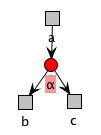
\includegraphics[scale=0.6]{graph_w_bds.png}}
\end{center}

Graphs with variable inputs and outputs (like spiders) can be represented using \textit{pattern graphs}. These graphs indicate sub-graphs which can be repeated many times by using \textit{bang-boxes} (by analogy to the ``bang'' operation $!(-)$ from linear logic). To make an input or an output variable, select the boundary vertex and click ``Bang vertices'' in the toolbox. We can then represent a spider of any arity as follows:
\begin{center}
  \tikzfig{red_spider} \ \ $:=$\ \ 
  \raisebox{-1.65cm}{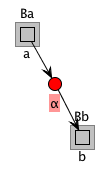
\includegraphics[scale=0.6]{spider_quanto.png}}
\end{center}

Note that bang-boxes have names as well. These and the names of boundaries can be changed by double-clicking on them. This will become important when defining rules. To define a rule, click the left arrow next to ``Toolbox'' to open the rules panel, and click ``New Rule''. Give the rule a name, and it will open as a pair of (empty) graphs, side-by-side. Click on the left or the right panel to focus on the LHS or RHS and edit the graph as before. Click the ``Save'' icon to save the rule back to the ruleset. Note that this will only succeed if you have input a valid rule. A valid rule must have:

\begin{enumerate}
  \item the same number of boundary vertices and bang-boxes on both sides,
  \item the same \textit{names} for boundary vertices and bang-boxes on both sides, and
  \item a \textit{compatible boxing} of boundary vertices. That is, if a boundary vertex named ``Va'' is in the box named ``Ba'' on the LHS, it must also be in the box named ``Ba'' on the RHS and vice-versa.
\end{enumerate}

For our purposes, we will only be placing single boundary vertices. Once rules are implemented, activate them using the button in the rule panel. Using the dropdown box below the toolbar, select a graph. Rules can be applied to a graph in one of two ways. The first is to apply rules manually, using ``Graph $>$ Show Rewrites''. The second is to apply rules automatically, using ``Graph $>$ Normalise'' or ``Graph $>$ Fast Normalise''.


\section*{Exercise 1: Implementing the Spider Laws}

The spider theorem for green dots looks like this:
\ctikzfig{spider_green}

Rather than implement the spider theorem as a single reduction rule, we can implement it as:

\begin{enumerate}
  \item A rule that merges adjacent dots of the same colour.
  \item A rule that removes self-loops.
  \item A rule that turns spiders with 1 input and 1 output
\end{enumerate}

Note the the first and second rule need to handle any number of inputs and outputs on the spiders. Bang-boxes can be used for this.

\medskip
\noindent{\color{blue} Implement the spider laws for red and green dots as rules (6 in total) in Quantomatic. Use these rules to simplify a graph consisting of red and green spiders, as well as some phases to a normal form.}
\medskip

\section*{Exercise 2: $\pi$-copy}

As a consequence of $\ket{z_\pi}$ being a classical point, the map $Z_\pi$ is copied through the red dot. In the process, any angle inside picks up a minus-1 phase shift.

\ctikzfig{pi_copy}

\medskip
\noindent{\color{blue} Implement the $\pi$-copy rule in Quantomatic.}
\medskip

However, once we implement this rule, we notice a problem! Consider graphs that look like this:

\ctikzfig{pi_copy_critical}

We now have a choice to apply the spider-merge rule to the two green vertices or to apply the copy rule to the red and green vertex. If we apply the spider rule, the copy will no longer be applicable and vice-versa. Therefore we have two distinct, equivalent normal forms. In rewriting lingo, this is called a \textit{critical pair}. We can close a critical pair by introducing a \textit{completion}.

\ctikzfig{pi_copy_completion}

\medskip
\noindent{\color{blue} Implement the completion above as a rule in Quantomatic. Show that the original $\pi$-copy rule is now redundant and remove it.}
\medskip

If we can close all critical pairs in a (terminating) rewrite system, it is possible to show that all normal forms are unique. That is, the system is \textit{confluent and terminating}.


\section*{Exercise 3: The CNOT Gate Using MBQC}

It is a well-known result that single-qubit unitaries and the CNOT gate are universal for quantum computing. In the Z/X calculus, we can write the CNOT gate as:
\begin{equation}\label{eq:cnot}
  \tikzfig{cnot}
\end{equation}

Recall the MBQC program from section~\ref{sec:mbqc}.

\[ M_2^0 M_4^0 E_{1,3} E_{2,3} E_{3,4} N_3 N_4 \]

\medskip
\noindent{\color{blue} Use the translation from section~\ref{sec:mbqc} to translate this program into a graph in Quantomatic, for measurement outcomes $\{ M_2^0 \rightarrow 0, M_4^0 \rightarrow 0 \}$. Implement enough rules from section~\ref{sec:zx} to normalise the measurement pattern into (\ref{eq:cnot}).}
\medskip

Even if we do not get outcome $00$, we can still produce a CNOT gate by performing single-qubit corrections.

\medskip
\noindent{\color{blue} For each of the other three outcomes, find red and green phases to apply to qubits 1 and 3 to produce a CNOT gate. Show that all four cases reduce to (\ref{eq:cnot}) in Quantomatic.}
\medskip

Let $M_{i,A}^\alpha$ be a measurement labelled $A$ of the $i$-th qubit at angle $\alpha$. Let $Z_j^A$ be the identity for the outcome $0$ of the measurement labelled $A$ and a $Z_\pi$ gate for outcome $1$. Define $X_j^A$ similarly. These are called \textit{conditional corrections}.

\medskip
\noindent{\color{blue} Using conditional corrections, write an MBQC program that produces the CNOT gate, regardless of the measurement outcomes.}
\medskip

\section*{Bonus: Implementing Single Qubit Unitaries}

Any single qubit unitary can be written using three phase gates, $U = Z_\alpha X_\beta Z_\gamma$.

\medskip
\noindent{\color{blue} Write an MBQC program that implements an arbitrary single qubit unitary. Show that for several combinations of outcomes that the program reduces to a composition $Z_\alpha X_\beta Z_\gamma$ in Quantomatic.}
\medskip

Note that measurement angles can be chosen based on previous measurement outcomes. This is known as \textit{feed-forward} in MBQC. The existence of these two programs shows that MBQC is as powerful as the circuit model.


\end{document}
